
\subsection{CubeSats}

Satélites pequenos, conhecidos como SmallSats, compreendem uma categoria de espaçonaves com massa inferior a 180 kg, esses satélites são classificados em diferentes categorias, dependendo de sua massa, conforme:
\begin{itemize}
    \item minissatélites (100-180 kg),
    \item microssatélites (10-100 kg),
    \item nanosatélites (1-10 kg),
    \item picosatélites (0,01-1 kg) e,
    \item femtosatélites (0,001-0,01 kg).
\end{itemize}
Esses sistemas têm ganhado destaque devido à sua modularidade e ao custo reduzido em relação a satélites convencionais \citep{nasa_smallsats_2024}.

\begin{figure}[H]
    \centering
    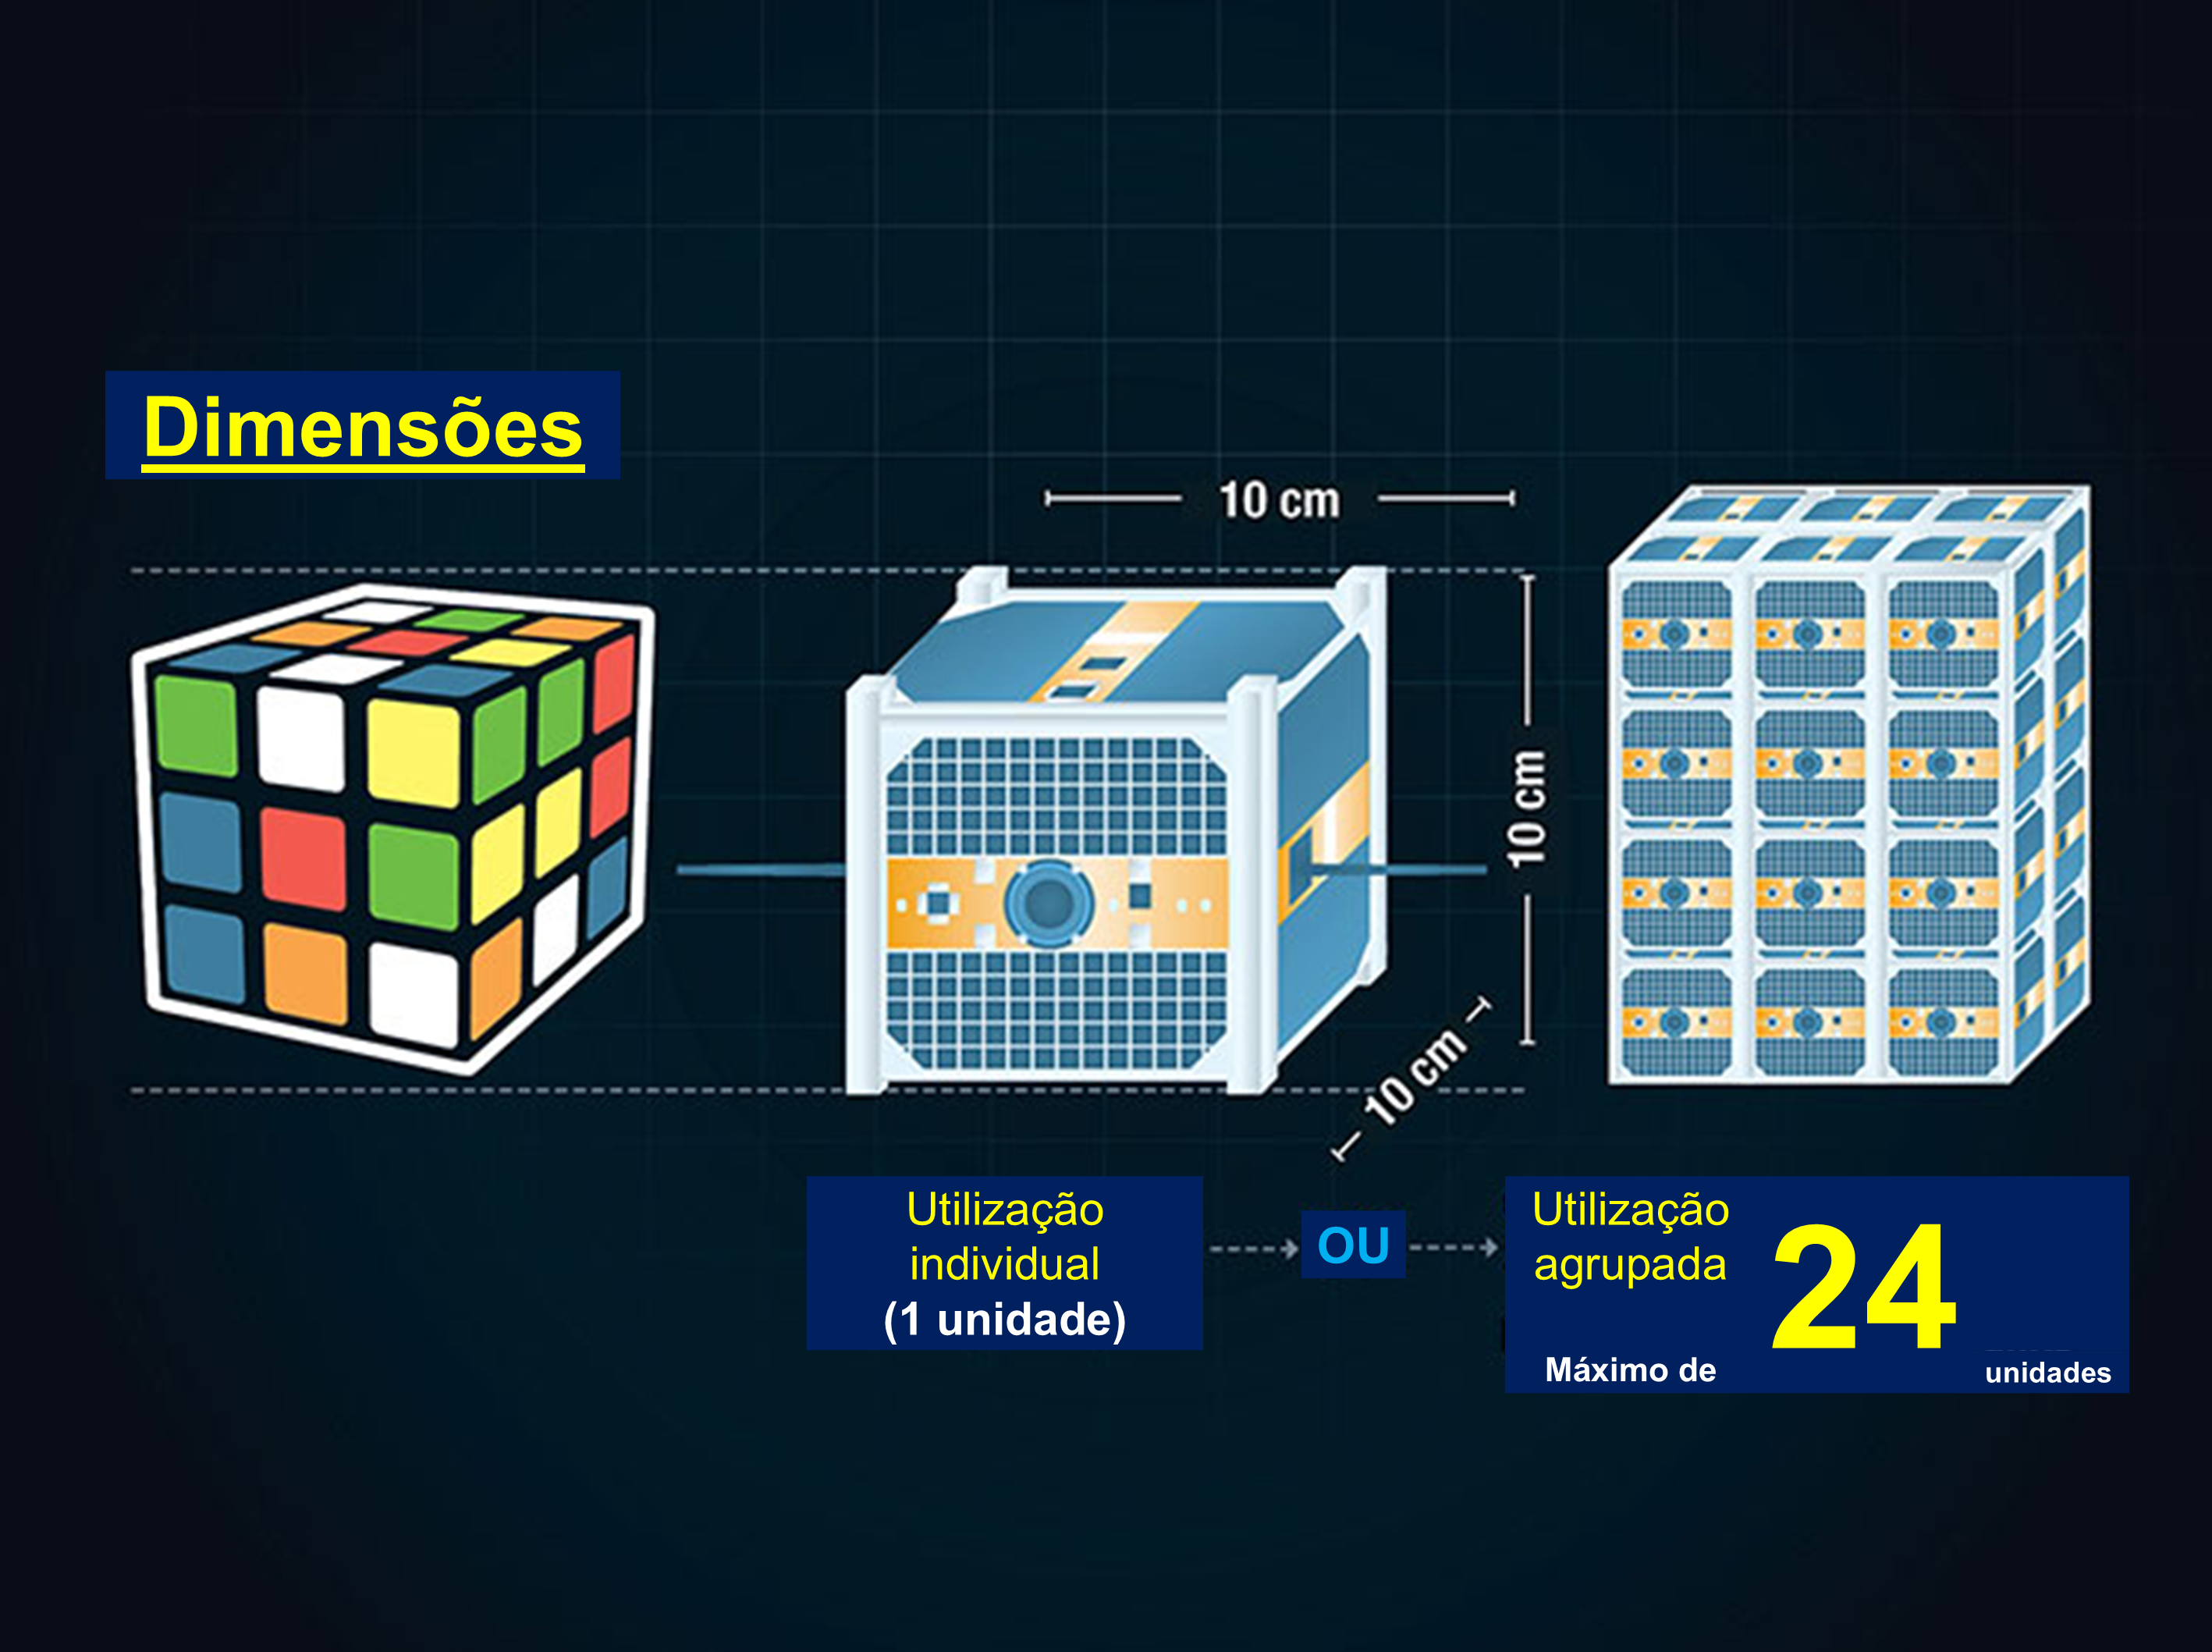
\includegraphics[width=0.75\linewidth]{Imagens/CubeSats_editado.png}
    \caption{CubeSats (adaptado pelo autor). Fonte: (\url{https://www.asc-csa.gc.ca/eng/satellites/cubesat/what-is-a-cubesat.asp})}
    \label{fig:enter-label}
\end{figure}

Ainda de acordo com \citep{nasa_smallsats_2024}, os CubeSats constituem uma subclasse de nanosatélites com um formato padronizado baseado em unidades cúbicas de 10x10x10 cm, denominadas "1U". De forma fácil e simplificada, essa configuração pode ser expandida para tamanhos maiores, como 1,5U, 2U, 3U, 6U e até 12U.
Os CubeSats foram desenvolvidos em 1999 pela California Polytechnic State University e Stanford University, e se consolidaram como uma plataforma para experimentos científicos, testes de novas tecnologias e demonstrações de conceitos avançados de missão, por consequência, o seu desenvolvimento levou à criação de uma indústria dedicada, com colaborações entre governo, indústria e academia.

\subsubsection{Exemplo de missão utilizando o CubeSat}

Um exemplo de missão que tinha o objetivo de expandir a ciência, como exemplo as demonstrações tecnológicas voltadas para novos métodos de propulsão, é a missão LightSail \citep{spencer_lightsail_2016}, desenvolvida pela The Planetary Society, que utilizou um CubeSat 3U para demonstrar a viabilidade da navegação espacial por vela solar. O primeiro CubeSat dessa missão foi lançado em 2015, com o objetivo de testar o processo de desdobramento da vela solar em órbita terrestre baixa, já a segunda missão, prevista para 2017, porém só foi realizada em junho de 2019 e esteve em órbita até novembro de 2022 conforme explica \citep{planetary_lightsail}, teve como propósito demonstrar o controle da vela solar e aumentar sua altitude orbital. A missão foi financiada por doadores privados e representa um marco no desenvolvimento de tecnologias alternativas de propulsão para pequenos satélites e reforça o potencial dos CubeSats para testar conceitos inovadores, especialmente aqueles voltados para exploração espacial sustentável. 

\begin{figure}[H]
    \centering
    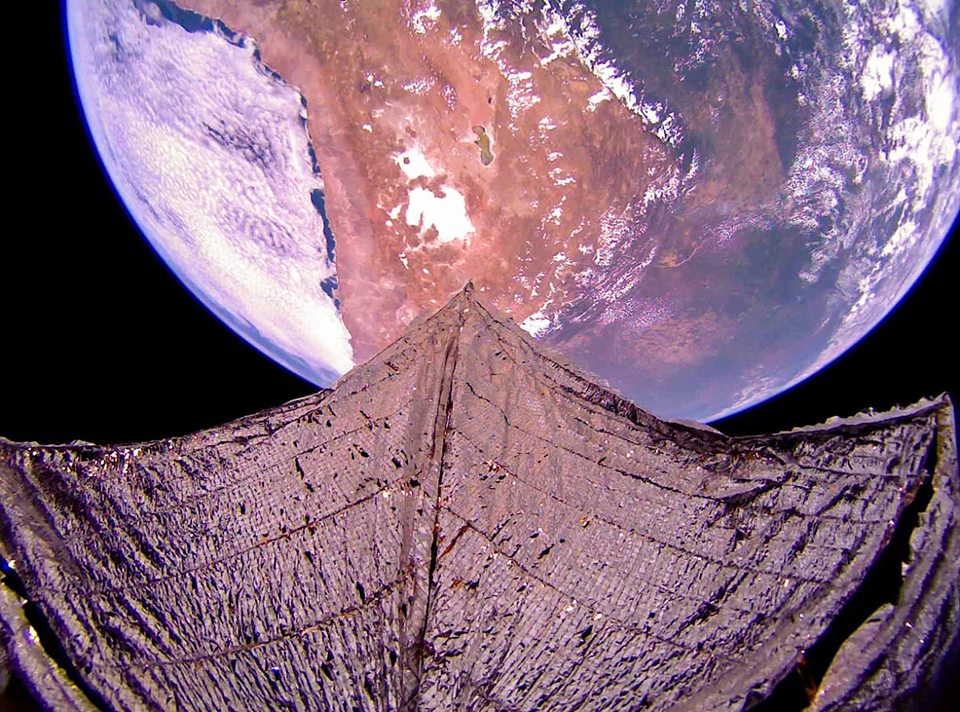
\includegraphics[width=0.75\linewidth]{Imagens/Lightsail.png}
    \caption{Última imagem do LightSail antes da reentrada terrestre. Fonte: Planeraty (\url{https://www.planetary.org/articles/lightsail-2-completes-mission})}
    \label{fig:LightSail}
\end{figure}